\documentclass[10pt,letterpaper,spanish,twoside]{report}

\usepackage{practica}
\usepackage{graphicx}
\usepackage{float}
\DeclareGraphicsExtensions{.bmp,.png,.pdf,.jpg}
\newcommand{\docdate}{
  \vspace{2em}
   \begin{flushright}
     Ciudad de México. \datedayname~\today.
   \end{flushright}
  \vspace{2em}
}

\begin{document}
\docdate

\begin{center}
 \textsc{\asignatura}\vspace{.2em}
\end{center}

\textsc{Manual del profesor}

\textsc{Práctica 2. aplicación de filtros analógicos tipo Butterworth pasa altas a señales biomédicas reales.}

\textsc{Objetivo:} Aplicar los conocimientos sobre el diseño de filtros Butterworth pasa altas para procesamiento de señales biomédicas reales simulando su adquisición en tiempo real.

\textsc{Actividades}
\begin{enumerate}
 \item Descargar el archivo de audio 'ECG resp.wav' de https://goo.gl/gKKAfd
 \item Obtener la FFT de la señal de electrocardiograma en el osciloscopio y localizar la frecuencia de corte que permitirá eliminar la interferencia de la señal.\\Como se puede observar en la figura%~\ref{contexto:FFT2},la interferencia pertenece a bajas frecuencias, alrededor de 2 Hz.
 \\INSERTAR IMAGEN DEL OSCILOSCOPIO 
 \item Para el diseño del filtro pasa altas orden 2 se sugiere utilizar una frecuencia de corte de 1 Hz. 
 \item Implementar el circuito que se muestra en la figura~\ref{contexto:PA2}, el cual contiene los valores de resistencias y capacitores que fueron obtenidos con la función bsk, en caso de cambiar la frecuencia de corte, es necesario volver a calcular estos valores
 \\También es posible observar en la ecuación~\eqref{FT_n2} la función de transferencia de dicho filtro, que es obtenida con la misma función bsk.
 \begin{equation}
 	H(s)=\frac{1.3s^2}{s^2+12.142s+8.877}\label{FT_n2}
 \end{equation}
 \begin{figure}[H]
 	\centering
 	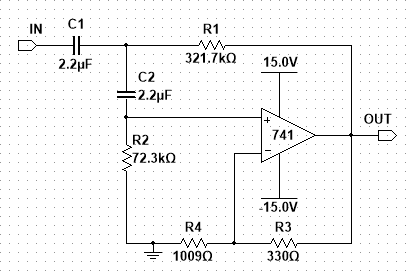
\includegraphics[scale=0.5]{PA2.PNG}
 	\caption{Circuito eléctrico de filtro pasa altas orden 2}
	\label{contexto:PA2}
 \end{figure}
 \item En la figura~\ref{contexto:RF_2} se observa la respuesta en frecuencia del filtro pasa altas orden 2
 \\Los datos obtenidos pueden consultarse en el archivo P1$\_$n2$\&$4$\_$caracterizacion.ipynb. \\Es posible observar que la frecuencia de corte se encuentra en alrededor de los 3 Hz 
  \begin{figure}[H]
 	\centering
 	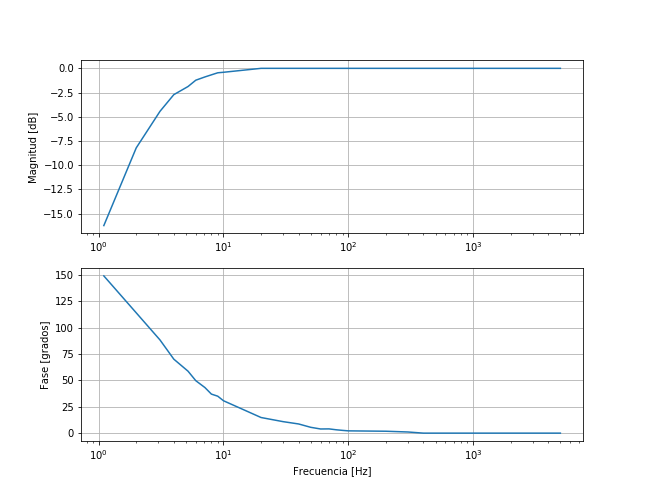
\includegraphics[scale=0.4]{RF_PA4.png}
 	\caption{Respuesta en frecuencia de filtro pasa altas orden 2}
 	%Falta cambiar la gráfica de la respuesta en frecuencia de orden 2
	\label{contexto:RF_2}
 \end{figure}
 \begin{enumerate}
  \item Una vez verificado que la frecuencia de corte se encuentra alrededor de la deseada, se procede a filtrar la señal, recordando que tiene que pasar por la etapa del preamplificador (simulador de paciente)
  \item Para evaluar la funcionalidad del circuito se recomienda hacer una comparación entre señal contaminada y filtrada, así también, de la FFT.
 \end{enumerate}  
 \item Para el diseño del filtro pasa altas orden 4 se sugiere utilizar una frecuencia de corte de 1.5 Hz.
 \item Implementar circuito de la figura~\ref{contexto:PA4}, que contiene los valores de capacitores y resistencias calculados con la función bsk.
 \\En la ecuación~\eqref{FT_n4} se presenta la función de tranferencia del filtro pasa altas orden 4.
 \begin{equation}
 	H(s)=\frac{1.4s^2}{s^2+17.806s+24.582} \frac{1.3s^2}{s^2+18.524s+10.199}\label{FT_n4}
 \end{equation}
 \begin{figure}[H]
 	\centering
 	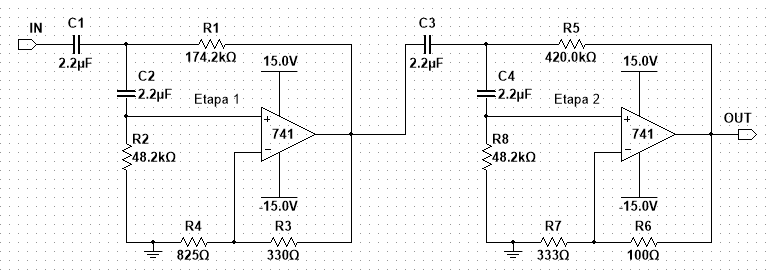
\includegraphics[scale=0.4]{PA4.PNG}
 	\caption{Circuito eléctrico de filtro pasa altas orden 4}
	\label{contexto:PA4}
 \end{figure}
 \item En la figura~\ref{contexto:RF_4} se puede observar la respuesta en frecuencia del filtro 4. Es posible observar que la frecuencia de corte se encuentra alrededor de los 3 Hz.
 \begin{figure}
 	\centering
 	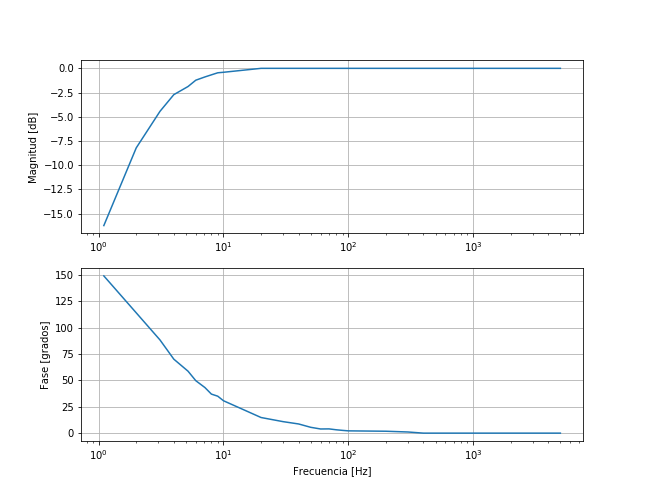
\includegraphics[scale=0.5]{RF_PA4.PNG}
 	\caption{Respuesta en frecuencia de filtro pasa altas orden 4}
 	\label{contexto:RF_4}
 \end{figure}
 \begin{enumerate}
 	\item Para observar la funcionalidad del circuito realizar la comparación entre señal contaminada y filtrada, así también, de la FFT. INSERTAR FIGURAS DE SEÑALES EN EL OSCILOSCOPIO
 \end{enumerate}
\end{enumerate}


%\textsc{Nota}
%\vspace{2em}
\vfill
\begin{flushright}
\textsc{Elaboró:\\
Ma. del Rosario Aguilar Cruz\\
Enrique Mena Camilo}
\end{flushright}

\end{document}